\documentclass[uplatex,a4j,12pt,twocolumn]{jsarticle}

\renewcommand{\baselinestretch}{0.99}
% 縦横のサイズ調整
\usepackage[margin=10mm]{geometry}
\usepackage[dvipdfmx]{graphicx,hyperref}
\usepackage{pxjahyper}
\usepackage{latexsym}
\usepackage{bmpsize}
\usepackage{url} % urlを参考文献で出力したいから使う
\usepackage{comment}
\usepackage{textcomp} % > などの記号を出力
\usepackage{here} % 画像を強制的に指定した箇所に出力
\usepackage{minted} % ソースコードのシンタックスハイライト
\usepackage{mdframed}
% 図の上下に微妙な隙間が出るので対策
\setlength\intextsep{3pt}
\setlength\textfloatsep{0pt}

\renewcommand{\listingscaption}{コード}  % キャプション名をコードに変更


\begin{document}


\title{InputMethodKitとTCAを使ったmacOS上で動作するIMEの開発}
\author{Tatsumi0000}
\date{}
\maketitle

\section{はじめに}\label{sec:intro}
私は普段Google IMEを使っているのですが、英単語をいい感じに補完してくれず、私が英単語を覚えるのが苦手なのも相まっていつも誤字脱字をしがちです。そこで、この課題を解決するために、英単語を補完するmacOS上で動作するIME、Raelize(れりーず)を開発しました。

Raelizeを開発するために、Appleが公式で提供しているInputMethodKit\cite{bib:about_inputmethodkit}を使って開発しました。実際に開発をしていく上で、ロジックが集中するIMKInputControllerにコードが集中し、コードの見通しが悪くなるという課題がありました。この課題に対しては、The Composable Architecture(TCA)\cite{bib:the_composable_architecture}を適用し解決しました。
他にも、IME開発特有のデバッグの煩わしさもあり、この課題に対しては、Raelizeをマルチモジュール構成にすることでデバッグ専用アプリの開発を容易にしたり、fastlane\cite{bib:fastlane}を用いた効率的なデバッグを行いました。

これらの開発体験を踏まえて本稿では、InputMethodKitとTCAを使ったIME開発や、マルチモジュール構成とfastlaneを用いた効率的なデバッグについて述べます。

今回使用した各ツールのバージョンを表\ref{table:version}に示します。
\begin{table}[h]
  \begin{center}
    \caption{各ツールのバージョン}
    \begin{tabular}{|l|r|} \hline
      ツール & バージョン \\ \hline
      macOS & 14.5 \\
      Xcode & 15.4 \\
      Swift & 5.10 \\
      The Composable Architecture & 1.9.2 \\
      Ruby & 3.3.0\\
      fastlane & 2.220.0 \\ \hline
    \end{tabular}
  \end{center}
\end{table}\label{table:version}

本稿の構成は以下の通りです。
第\ref{sec:abount_inputmethodkit}章ではInputMethodKitについて述べます。第\ref{sec:the_composable_architecture}章ではThe Composable Architecture(TCA)について述べます。第\ref{sec:use_imk_and_tca}章ではInputMethodKitとTCAを使ったIME開発について述べます。第\ref{sec:multi_module_and_fastlane}章ではマルチモジュール構成とfastlaneを用いた効率的なデバッグについて述べます。第\ref{sec:conclusion}章では本稿のまとめ述べます。

解説に使用するコードは、\url{https://github.com/Tatsumi0000/Raelize/tree/main}で公開しています。

\section{InputMethodKit}\label{sec:abount_inputmethodkit}
InputMethodKitについて述べます。InputMethodKitは、macOSでIMEを開発するためのフレームワークで、macOSのIMEとして動作するアプリケーションを開発することができます。

InputMethodKitは、主に以下の3つのクラスを使って開発します。
\begin{itemize}
    \item IMKServer
    \begin{itemize}
        \item 入力メソッドへのクライアント接続を管理するクラス\cite{bib:imkserver}
    \end{itemize}
    % \newpage
    \item IMKCandidates
    \begin{itemize}
        \item 候補ウィンドウを表示するためのクラス\cite{bib:imk_candidates}
    \end{itemize}
    \item IMKInputController
    \begin{itemize}
        \item 入力メソッドのテキスト入力を制御するクラス\cite{bib:imk_input_controller}。このクラスをオーバライドしてIMEのロジックを実装する
    \end{itemize}
\end{itemize}


\section{The Composable Architecture}\label{sec:the_composable_architecture}
The Composable Architecture(TCA)について述べます。TCAは、Point-Freeが開発しているライブラリで一貫性のあるコードを書くことができます。TCAは、UIKitやSwiftUIを使っていないアプリケーションに対しても適用が可能で、今回はIMKInputControllerにコードが集中するという課題を解決するために使用しました。

\section{InputMethodKitとTCAを使ったIME開発}\label{sec:use_imk_and_tca}
InputMethodKitとTCAを使ったIME開発について述べます。以下のような実装をすることで、コードの見通しをよくしました。
 
\begin{itemize}
  \item IMKInputControllerのイニシャライザでTCAのStateを監視し、状態に応じてIMKCandidatesを操作
  \item IMKInputControllerの各メソッド内で、TCA側のActionを呼び出す
\end{itemize}
コード\ref{listings:state}に、RealizeでのState、コード\ref{listings:initial_state}にIMKInputControllerのイニシャライザでStateを監視するコード例を示します。

\begin{listing}[h]
  \begin{minted}[breaklines]{swift}
@ObservableState
public struct State: Equatable {
  /// IME の入力モード
  var raelizeState: RaelizeState
  /// ユーザに表示する補完候補一覧
  var candinates: [String] = []
  /// ユーザが入力している文字
  var inputWord: String = ""
  /// 単語リストのファイル名
  var fileName: String = ""
  /// ユーザが選択した補完候補
  var insertText: String = ""
  /// ユーザが選択した補完候補の文字列
  var selectedWord: String = ""
  /// IME に対してユーザが起こしたイベント
  var candidateEvent: NSEvent? = nil
}
  \end{minted}
  \caption{RealizeでのState例}\label{listings:state}
\end{listing}

\begin{listing}[h]
  \begin{minted}[breaklines]{swift}
initialState: RaelizeIMKReducer.State(raelizeState: .inputMode),
  reducer: { RaelizeIMKReducer() })
  observe {
    // ユーザが未入力もしくは補完候補がない場合は候補ウィンドウを非表示
    if self.store.candinates.isEmpty || self.store.inputWord.isEmpty {
      self.candidates.hide()
    // 候補ウィンドウ内容を更新してから表示
    } else {
      self.candidates.update()
      self.candidates.show()
    }
  }
  \end{minted}
  \caption{IMKInputControllerのイニシャライザでのStateを監視する例}\label{listings:initial_state}
\end{listing}
次にIMKInputControllerで使用したメソッドと一緒に、どのようにTCAを組み合わせて実装したか述べます。
\subsubsection{handle(\_ event: NSEvent!, client sender: Any!) -\texttt{>} Bool}
このメソッドは、ユーザがキーボードを操作した際に呼ばれるメソッドです。eventにユーザが操作したイベントが格納されているので、このイベントに応じてIMEの状態(RaelizeState)を切り替えます。コード\ref{listings:handle}に、コード例を示します。
\begin{listing}[h]
  \begin{minted}[breaklines]{swift}
public override func handle(_ event: NSEvent!, client sender: Any!) -> Bool {
  guard let event = event else { return false }
  // 受け取ったイベントに応じて状態を切り替える Action を呼び出す
  store.send(.handleRaelizeState(event))
  switch store.raelizeState {
  // 何もないモード
  case .neutralMode:
    return false
  // 文字入力 or 補完ウィンドウ操作モード  
  case .inputMode, .operationMode:
    return true
  }
}
  \end{minted}
  \caption{handleのコード例}\label{listings:handle}
\end{listing}

\subsubsection{candidates(\_ sender: Any!) -\texttt{>} [Any]!}
補完ウィンドウに表示する内容を返り値で返すメソッドです。StoreのStateを返すだけにしています。コード\ref{listings:candidates}に、コード例を示します。
\begin{listing}[h]
  \begin{minted}[breaklines]{swift}
public override func candidates(_ sender: Any!) -> [Any]! {
  // candinates自体は[String]型です
  return self.store.candinates
}
  \end{minted}
  \caption{candidatesのコード例}\label{listings:candidates}
\end{listing}

\subsubsection{candidateSelected(\_ candidateString: NSAttributedString!)}
補完候補を選択した際に呼ばれるメソッドです。選択した文字列をActionに渡します。コード\ref{listings:candidate_selected}に、コード例を示します。
\begin{listing}[h]
  \begin{minted}[breaklines]{swift}
public override func candidateSelected(_ candidateString: NSAttributedString!) {
    self.store.send(.insertText(
      candidateString.string
    ))
}
  \end{minted}
  \caption{candidateSelectedのコード例}\label{listings:candidate_selected}
\end{listing}

\subsubsection{candidateSelectionChanged(\_ candidateString: NSAttributedString!)}
補完ウィンドウの選択肢を切り替えたとき呼ばれます。コード\ref{listings:candidate_selection_changed}に、コード例を示します。
\begin{listing}[h]
  \begin{minted}[breaklines]{swift}
public override func candidateSelectionChanged(_ candidateString: NSAttributedString!) {
    guard let candidateString = candidateString else { return }
    self.store.send(.selectedWord(
      candidateString.string
    ))
}
  \end{minted}
  \caption{candidateSelectionChangedのコード例}\label{listings:candidate_selection_changed}
\end{listing}

\section{マルチモジュール構成とfastlaneを用いた効率的なデバッグなど}\label{sec:multi_module_and_fastlane}
マルチモジュール構成とfastlaneを用いた効率的なデバッグについて述べます。Swift Package Manager(SPM)を使ったマルチモジュール構成にすることで、単語を補完するためのロジックをデバッグ専用のアプリが開発しやすくなりました。単語補完ロジックをデバッグするだけのアプリを開発しやすくなりました。図\ref{fig:raelize_architecture}にRaelizeのモジュール構成を示します。

\begin{figure}[h]
  \begin{center}
      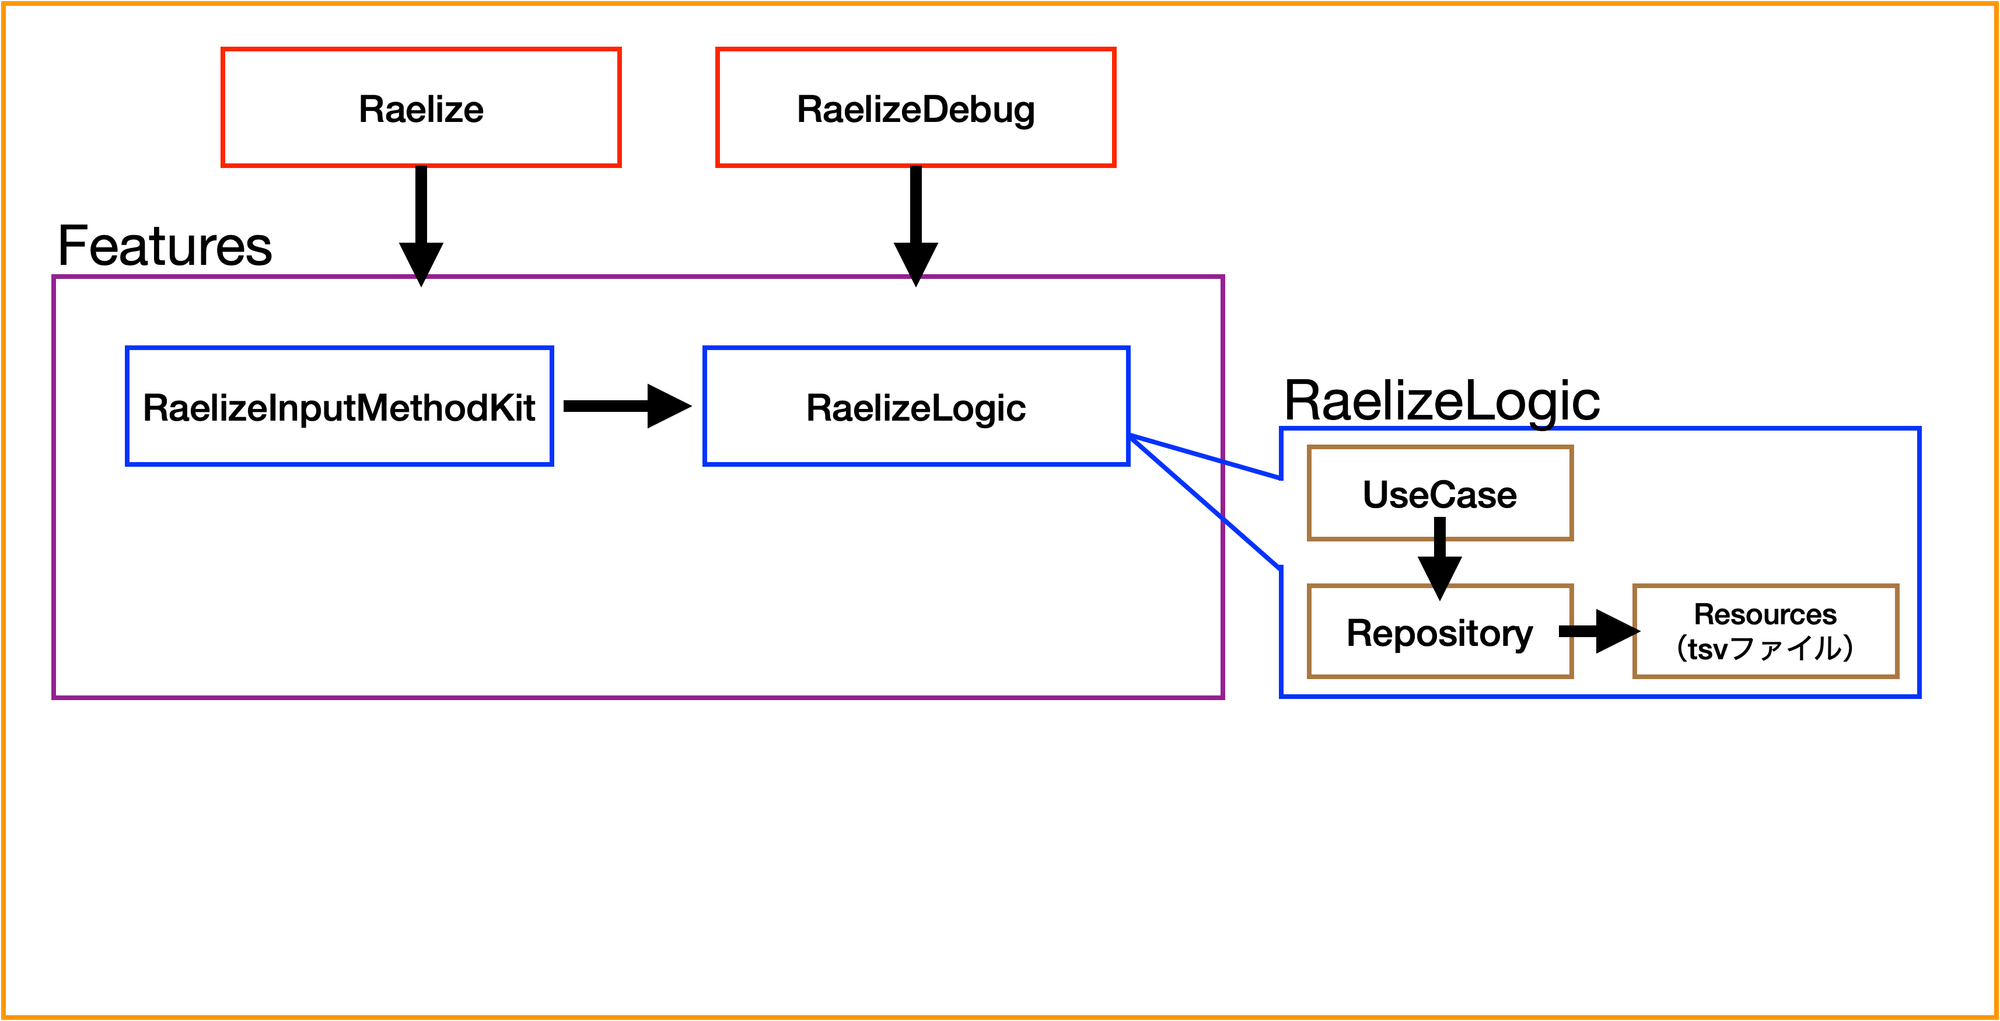
\includegraphics[width=7cm]{image/architecture.png}
      \caption{Raelizeのモジュール構成}
      \label{fig:raelize_architecture}
  \end{center}
\end{figure}

また、fastlaneを用いたビルドの自動化を行いました。IMEは通常のアプリケーションと異なり、ビルドしたファイルを特定のディレクトリに配置し、IMEのプロセスをkillすることでようやく使うことが出来ます\cite{bib:input_method_kit_tips}。これを毎回手動で実施するのは大変なので、fastlaneを用いて自動化しました。実際のコード例をコード\ref{listings:fastlane}に示します。

\begin{listing}[h]
  \begin{minted}[breaklines]{ruby}
default_platform(:mac)
platform :mac do
  desc "Build macOS App"
  lane :app_build do
  ime_path = "/Library/Input Methods"
    build_mac_app(
    configuration: "Debug",
    export_method: "development",
    scheme: "Raelize",
    output_directory: "#{ENV["HOME"]}#{ime_path}",
    clean: true
    )
    sh("pkill", "Raelize")
  end
end
  \end{minted}
  \caption{fastlaneを使ったビルド自動化}\label{listings:fastlane}
\end{listing}

コード\ref{listings:fastlane}を実行することで、IMEを使うことができるのですが、稀にIMEが起動しない場合があります。この場合は、PCをログアウト後再ログインすることで解決します。

IME開発中にprintデバッグをしたい場合はprintを使うのではなく、NSLogを使うことで、ログをConsoleアプリ\cite{bib:console}に出力します。そのまま使うとIME以外のログも大量に出力されて、分かりにくいため、Consoleアプリの右上からフィルタリング(アプリ名などで)を行い、IMEのログだけを出力することをおすすめします。

\section{おわりに}\label{sec:conclusion}
本稿では、InputMethodKitとTCAを使ったIME開発と、マルチモジュール構成、fastlaneを用いた効率的なデバッグについて述べました。InputMethodKitとTCAを一緒に使い開発することでコードの見通しをよくしつつ開発することが出来ました。他にもマルチモジュール構成とfastlaneを用いることで、効率的なデバッグを行うことができました。

%参考文献
\bibliography{iosdc2024} 
\bibliographystyle{junsrt} 

\end{document}
